%!TEX root = /Users/stefano/Documents/Bonsai Club/TWBC/twbc.tex

% \begin{figure*}[!hbp]
% \centering
% 
\includegraphics[width=1.0\textwidth]{2025_03/chris_durne.jpg}
% \centerline{\emph{Chris standing in front of the gold medal Bonsai display he curated at the Chelsea Flower Show.}}
% \end{figure*}

\headline{{\textbf{\Large\sffamily Bonsai Roots:}}\\
          {\textbf{\large\sffamily Meet the Members of TWBC}}}
\label{2025-04-roots}

\noindent
Welcome back to \textit{Bonsai Roots}, our monthly column where we introduce the wonderful members who bring life and energy to the Twickenham Bonsai Club. This feature aims to deepen connections within our community and provide potential new members with a closer look at the people who shape our vibrant club. 

This month, we're thrilled to feature \textbf{Martin Redfern}, a dedicated bonsai enthusiast whose journey is as inspiring as it is heartfelt. Martin's story is a testament to how bonsai can be more than just a hobby---it can be a source of confidence, connection, and personal growth.

\begin{itemize}
    \item \textbf{What's your name and where in the country do you live?}
    
    \emph{Hello, I'm Martin Redfern, and I live in Feltham, Middlesex.}

    \item \textbf{What are your favourite species of tree and why?}
    
    \emph{I don't really have a specific favourite. I just admire the beauty that each species of tree can become when it's made into a bonsai. Every tree has its own unique charm.}

    \item \textbf{What aspect of bonsai do you enjoy?}
    
    \emph{I enjoy being able to keep my trees alive (laughs) and watching them grow. There's something incredibly satisfying about nurturing a tree and seeing it thrive.}

    \item \textbf{What aspects of bonsai do you find most challenging?}
    
    \emph{I find a lot of things challenging, especially wiring and the art of styling. Knowing where to begin can be daunting, but it's all part of the learning process.}

    % \begin{window}[2,l,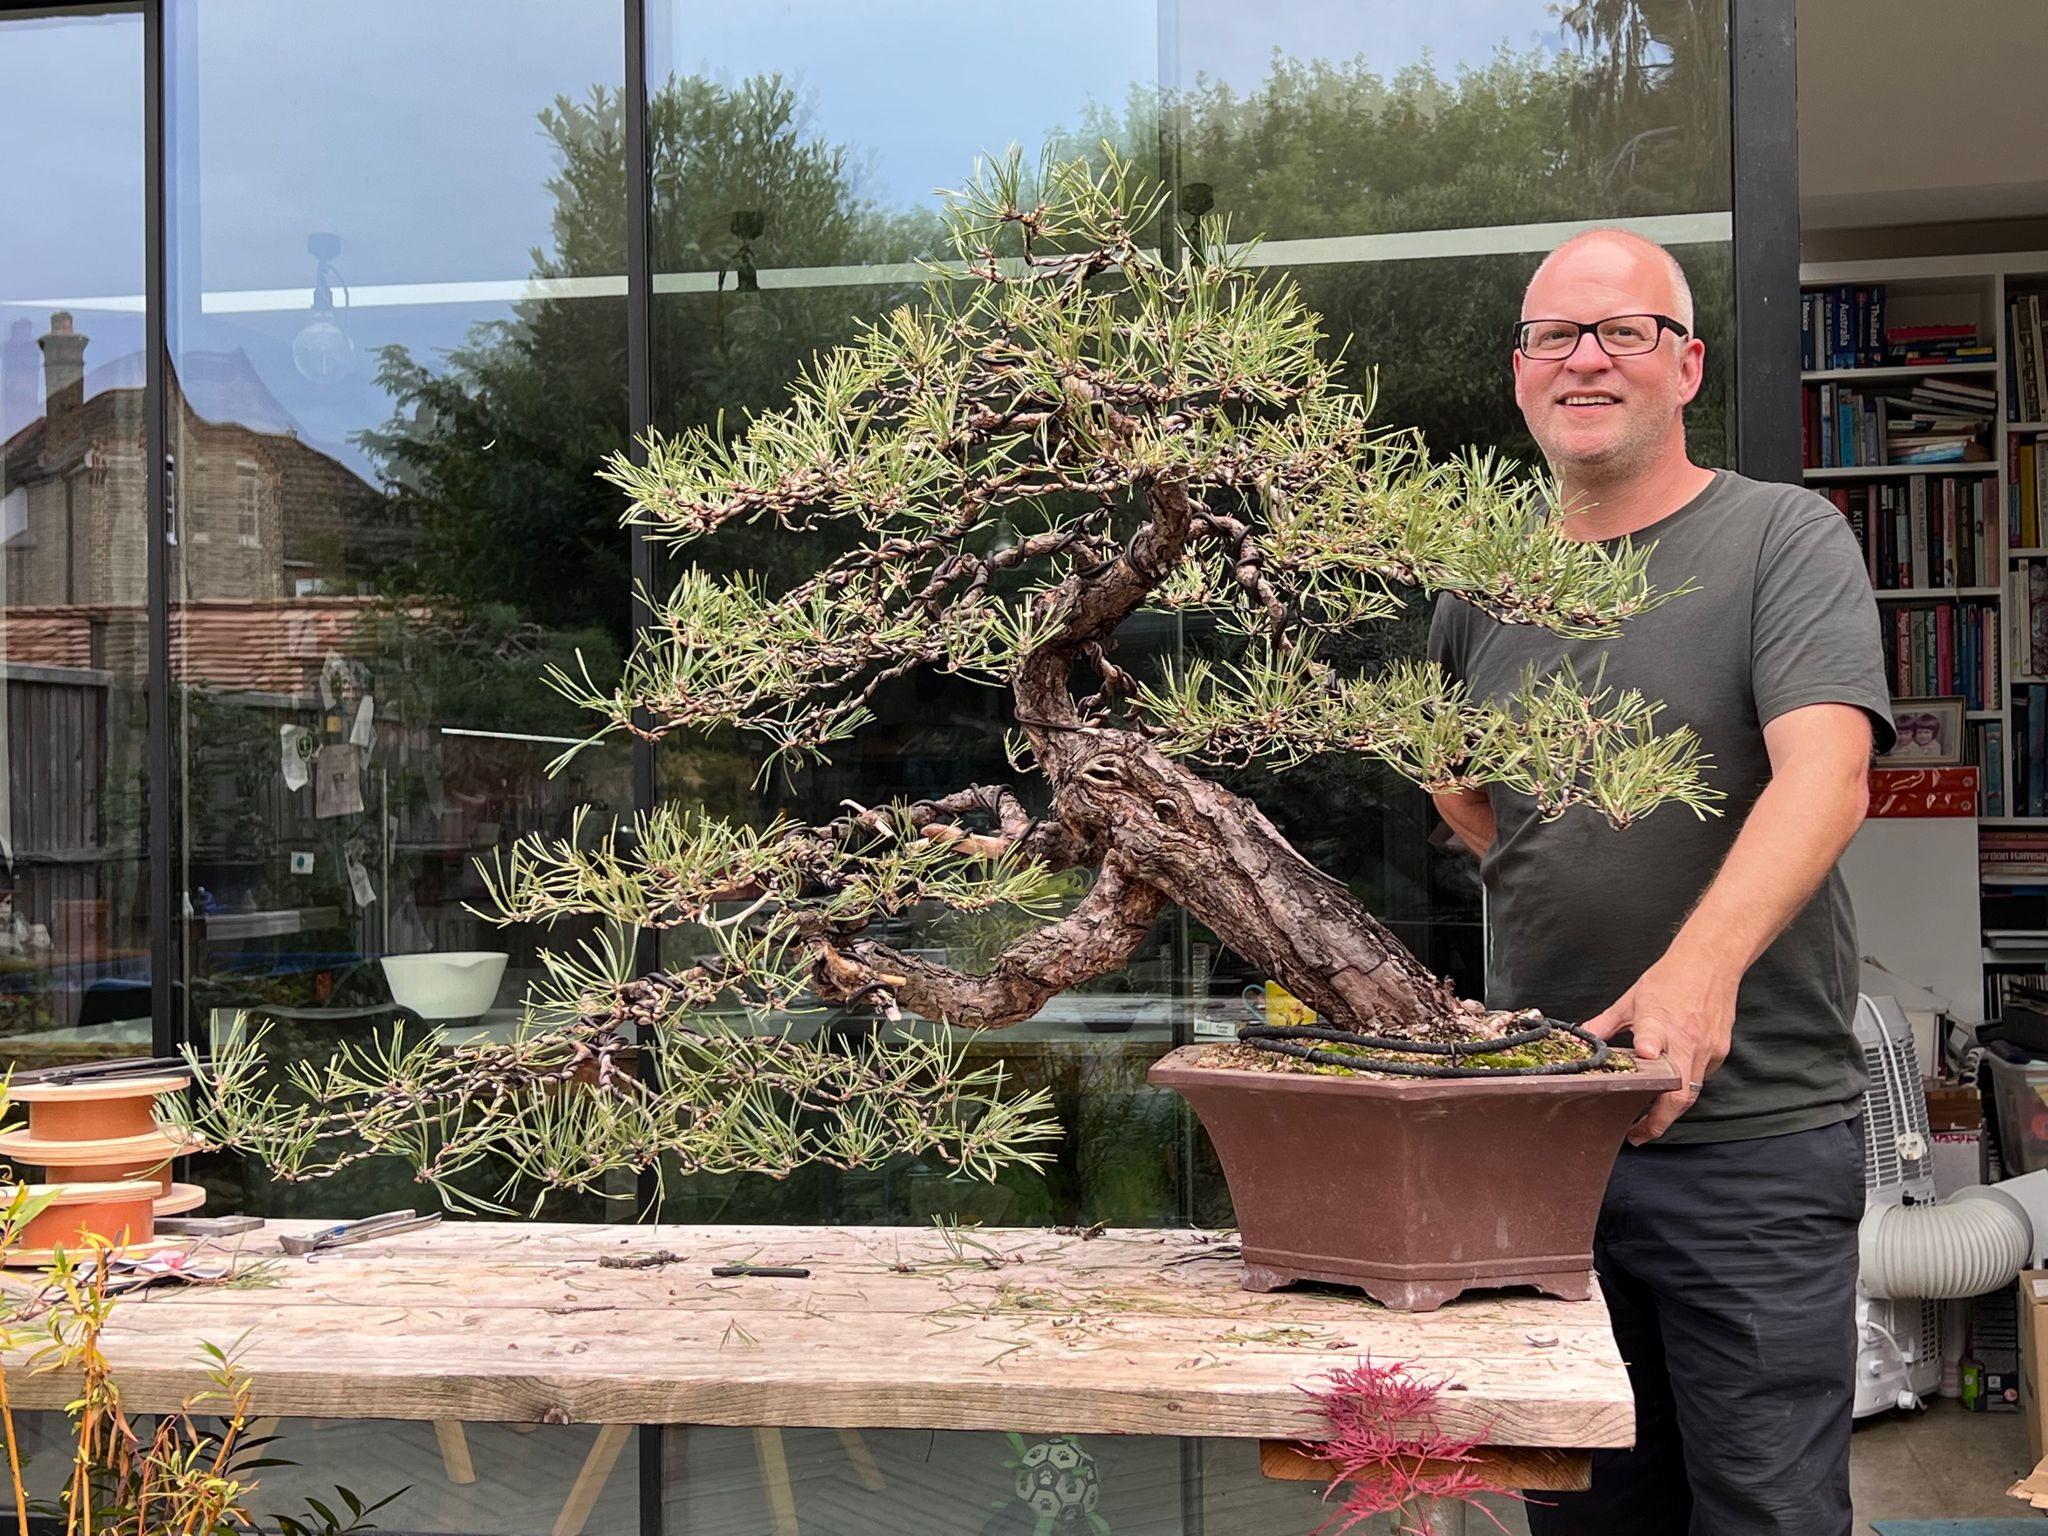
\includegraphics[width=1.0\columnwidth]{2025_03/res/roots_mark_edwards.jpeg},\centerline{\emph{Mark with his cherished Scots Pine, a tree with history.}}]
    % \end{window}
    % \columnbreak

    \item \textbf{Who or what inspires you throughout your bonsai journey?}
    
    \emph{I must admit that watching YouTube videos has helped me learn a lot. Joining the Twickenham Bonsai Club has also been a major step for me. The friendly and welcoming nature of the group inspires me to improve.}

    \item \textbf{How long have you been interested in bonsai?}
    
    \emph{I've had an interest in bonsai for about three years, ever since receiving my first tree. That was the start of it all.}

    % \begin{window}[2,l,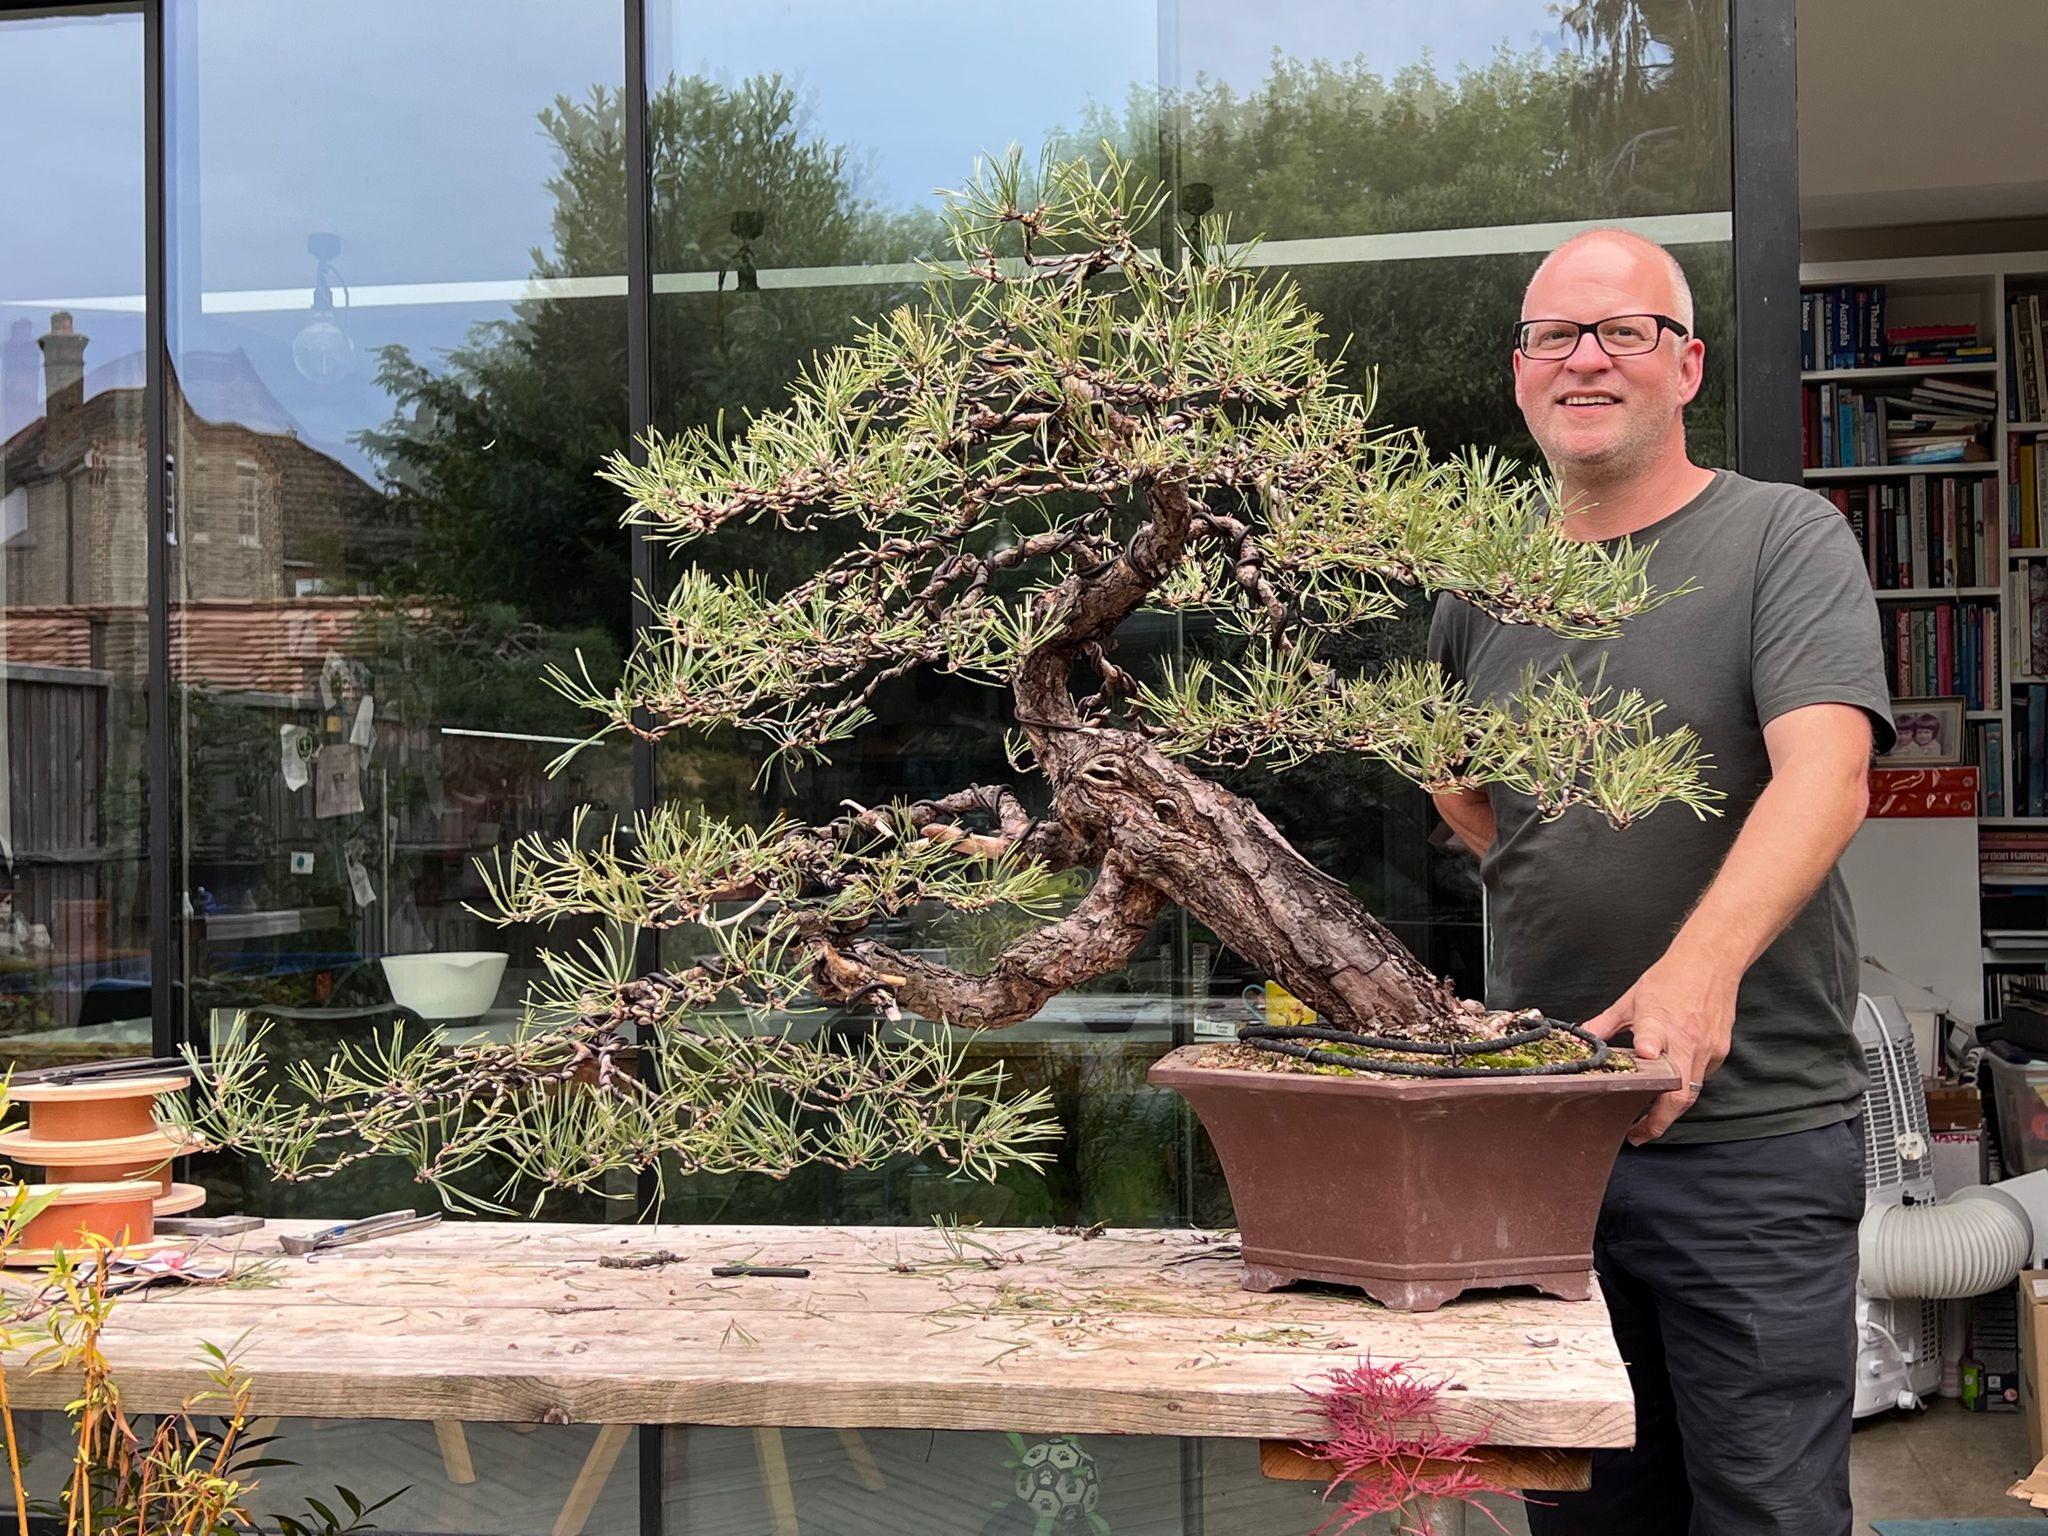
\includegraphics[width=1.0\columnwidth]{2025_03/res/roots_mark_edwards.jpeg},\centerline{\emph{Mark with his cherished Scots Pine, a tree with history.}}]
    % \end{window}

    \item \textbf{What stimulated your interest in bonsai?}
    
    \emph{I owe my interest in bonsai to my son, who sparked my passion by giving me my very first tree---a Cotoneaster---as a Father's Day gift.}

    \item \textbf{If you could give someone new to bonsai any tips, what would it be?}
    
    \emph{I would encourage them to find a supportive and friendly community, like a bonsai club, as it can be very helpful in building confidence and learning the craft.}

    \item \textbf{Why do you enjoy being part of TWBC, and do you have any ideas or suggestions for the club's future?}
    
    \emph{I enjoy being part of Twickenham Bonsai Club because it is a friendly and welcoming group. As someone who struggles with socializing and self\--confidence, the support from members has been invaluable to me.}

    \item \textbf{One word to describe what bonsai means to you?}
    
    \emph{Enjoyable.}

    \item \textbf{What are your future goals regarding your own trees and learning more about the hobby?}
    
    \emph{I hope to become a better bonsai keeper and continue watching my trees progress and flourish. It's all about growth---for the trees and for me.}

    \item \textbf{How would you like to see your bonsai journey progress in the future?}
    
    \emph{I want to use bonsai as a way to build confidence and gain a sense of achievement, no matter how big or small. Having a tree chosen for the winter show was a great boost, and I hope to continue growing in both skill and confidence.}

\end{itemize}

\noindent
We hope you've enjoyed getting to know Martin and his bonsai journey. His story is a beautiful reminder of how bonsai can bring people together, build confidence, and create a sense of belonging. Stay tuned to \emph{Bonsai Roots} for more member stories in the coming months!

\begin{center}
    $\cdots$
\end{center}

% \noindent
\emph{If you'd like to be featured in a future edition of Bonsai Roots or know someone who should, drop us a line! We're always eager to share the stories of our wonderful members.}

\begin{window}[2,l,\includegraphics[width=1.0\columnwidth]{2025_04/res/roots_martin_redfern.png},\centerline{\emph{Bonsai whispers and carp dances in Martin’s garden retreat.}}]
\end{window}
% \columnbreak

\closearticle
\columnbreak
